\chapter{CONCLUSIONS}
\label{chap:review}

\section{Encountered issues}

Although the app development has been smooth, there have been some difficulties. These are the ones that stand out the most:

\begin{itemize}
    \item \textbf{Duplicate subjects}: When I implemented the subject's creation, some subjects were added 2, 3, or even 4 times to the database with the same information. It turned out to happen when the user clicked the create button, the app sent the subject to the database and once it got an affirmative reply it closed the create screen. But if the connection was slow this could take some seconds, and impatient users clicked the create button multiple times, leading to copies in the database. I fixed it by freezing the screen until the response was received (Fig. \ref{fig:freeze}). The cause of this problem was very difficult to find because I could not recreate it, and I spend extra time on it.
    \item \textbf{Auto-update subject's structure}: The subject's object structure changed over the course of the project, adding, deleting, renaming, and moving its fields to accommodate new functionalities. Each time I had to change the specification I had to parse the old object structure into the new one of all the subject's in the database and the localStorage of the user's device. This made me spend an unplanned time on it.
    \item \textbf{Edit subject grid}: The evaluation grid inside the edit subject screen (Fig. \ref{fig:edit}) was quite complex to implement because the rows had to be added and deleted and at the end all the information parsed from the inputs into a JSON object. I underestimated this task, but in the end, I could do it.
    \item \textbf{Instant search}: Firebase doesn't provide full-text search \cite{algolia-why}, so I had to use Algolia. The problem was that Algolia requires a copy of the entire database, the usual approach is to make the copy at the beginning, and for future entries add them in both databases (Firebase's and Algolia's). But Firebase's free plan doesn't allow to run a function that sends data to an external source and I needed a workaround. My workaround was to set up a cron job in Heroku that runs every day and sends the new records to Algolia. This problem was a headache for some time because I wasn't coming up with any solution.
\end{itemize}

\noindent
In the end, all these problems were successfully solved.

\vfill
\begin{figure}[h!]
    \center
    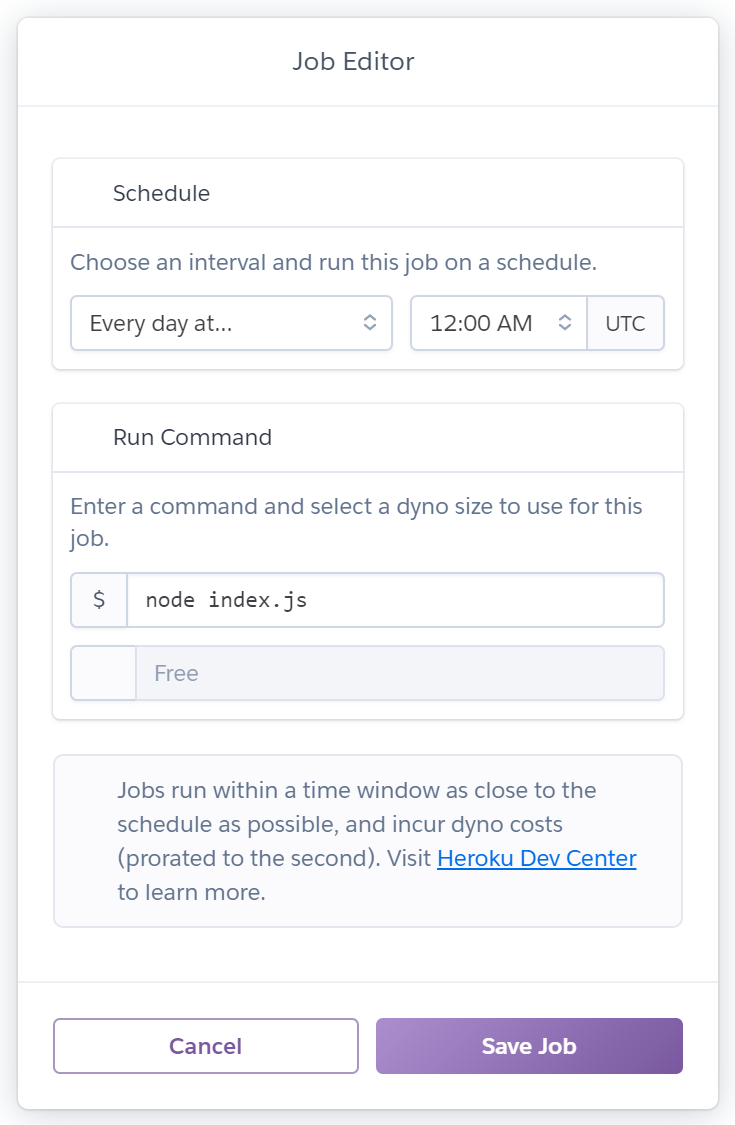
\includegraphics[width=0.35\linewidth]{media/heroku.png}
    \caption{Heroku cron job configuration}
\end{figure}
\vfill

\clearpage\newpage
\section{Accomplished objectives}

All of the objectives of the project defined in section \ref{sec:objectives}, have been correctly achieved. These are justifications:
\begin{itemize}
    \item \textbf{Add functionalities}: 
        The app now has, shared subjects database, many small details, create and edit subjects, it's installable...
    \item \textbf{Migrate code to a JavaScript task runner or bundler.}: 
        The app now uses Gulp.
    \item \textbf{Improve UI design}: 
        Now the subjects are displayed in beautiful cards in the dashboard and all other components follow the same style. All the user interface is explained in section \ref{sec:ui}.
    \item \textbf{Brand design}: 
        GradeCalc now has a defined brand and its style is used consistently. The details are explained in section \ref{sec:brand}.
    \item \textbf{Bug fixing}: 
        The app now doesn't have any critical bugs and can be used without problems.
    \item \textbf{Add tests to the code}: 
        Tests have been defined and added to the code. They are explained in chapter \ref{chap:testing}.
    \item \textbf{Implement Continuous Integration and Deployment}: 
        The app has both Continuous integration and deployment, and it takes advantage of its benefits. The setup is explained in chapter \ref{chap:devops}.
    \item \textbf{Implement users accounts}: 
        The app now uses Firebase and users can sign-up with Google to synchronize their grades, among other things. 
\end{itemize}




\clearpage\newpage
\section{Technical competences' accomplishment}
The technical competencies defined for this project are the following.

\subsection*{CES1.4: To develop, maintain, and evaluate distributed services and applications with network support. {\normalfont\normalsize [In depth]}}

The application is based in web technologies (section \ref{sec:stack}), so it has intrinsic network support. 
\begin{itemize}
    \item \textbf{Develop}: In chapter \ref{chap:design}, all the application's software is explained and this is how it has been developed.
    \item \textbf{Maintain}: In chapter \ref{chap:post}, the maintenance of the app is explained.
    \item \textbf{Evaluate}: In chapter \ref{chap:testing}, it is explained how the app is tested and evaluated.
\end{itemize}

\noindent
This competence has been accomplished successfully.

\subsection*{CES1.5: To specify, design, implement and evaluate databases. {\normalfont\normalsize [Enough]}}

\begin{itemize}
    \item \textbf{Specify}: In section \ref{sec:database}, the database is specified in both UML and TypeScript to provide a clearer understanding.
    \item \textbf{Design}: Also section \ref{sec:database}, explains that the database is designed specifically for the app to use the advantages of noSQL.
    \item \textbf{Implement}: The final app uses the defined database.
\end{itemize}

\noindent
This competence has been accomplished successfully.

\subsection*{CES2.1: To define and manage the requirements of a software system. {\normalfont\normalsize [Enough]}}

In chapter \ref{chap:requirements}, the requirements of the software system have been defined and managed.

This competence has been accomplished successfully.


\subsection*{CES1.2: To solve integration problems in function of the strategies, standards and available technologies. {\normalfont\normalsize [A little bit]}}

The integration problems that the application faced where:
\begin{itemize}[noitemsep]
    \item Connecting and using Firebase's database.
    \item Using Google's authentication service.
    \item Bundling the web app into an android app with android studio.
    \item Setting up continuous integration and continuous deployment.
    \item Setting up Gulp as a bundler and using libraries.
\end{itemize}

\noindent
These problems were solved in accordance with the:
\begin{itemize}[noitemsep]
    \item \textbf{Strategies}: In section\ref{sec:patterns}, the used design patterns are showcased.
    \item \textbf{Standards}: The standards are taken for granted, the app uses popular and loved by the community technologies that use well-established standards. Like using JSON in the request's body, or using standard UI components like popups, notification banners, cards...
    \item \textbf{Available technologies}: In section\ref{sec:stack}, the technologies are chosen, taking into consideration the requirements of section \ref{chap:requirements}.
\end{itemize}

\noindent
This competence has been accomplished successfully.

\subsection*{CES1.7: To control the quality and design tests in the software production. {\normalfont\normalsize [A little bit]}}

\begin{itemize}[noitemsep]
    \item \textbf{Control the quality}: In section \ref{sec:survey}, the satisfaction survey checks the quality.
    \item \textbf{Design tests}: In chapter \ref{chap:testing}, the tests are designed.
\end{itemize}

\noindent
This competence has been accomplished successfully.


\subsection*{CES2.2: To design adequate solutions in one or more application domains, using software engineering methods which integrate ethical, social, legal and economical aspects. {\normalfont\normalsize [A little bit]}}

GradeCalc has been designed to provide value to the students from the beginning (Chapter \ref{chap:intro}). This is how it integrates other domain aspects:
\begin{itemize}
    \item \textbf{Social}: It modifies the way students study for exams, letting them optimize more their time and invest the saved time into other activities. 
    \item \textbf{Ethical}: The app itself is completely transparent. It can be argued that the app makes students lazier by aiming for lower grades, but the reality is that there are many legit use cases of the app. For example, if a subject doesn't add value to a student, he may spend the minimum time on it and use the saved time in other, more valuable, activities. Or another example, a student that failed an exam at the beginning of the course will study harder to pass, making him learn more.
    \item \textbf{Legal}: It complies to the applicable legislation, it's explained in section \ref{sec:laws}.
    \item \textbf{Economical}: The project's costs are kept to the minimum, so this is an aspect that has been present when choosing the technologies (section \ref{sec:stack}) and also taken into account in the budget (section \ref{sec:budget}).
\end{itemize}

\noindent
This competence has been accomplished successfully.


\clearpage\newpage
\section{Integration of knowledge}

Most of the technical knowledge used in this project has been acquired by self-learning, especially watching a lot of YouTube videos, reading articles, doing prior projects, and searching problems in stack-overflow between many more things. Nonetheless, I learned a solid base from the bachelor course in FIB UPC. These are the subjects that taught me relevant knowledge for this project.

\begin{itemize}
    \item \textbf{ASW}: Understanding the usual architecture for web applications is a must to build one. It may have been the most relevant subject for this project, although it didn't go deep into the topic as I would have liked.
    \item \textbf{IDI}: The design principals they taught were really useful when designing an accessible and clean UI.
    \item \textbf{AS}: I learned how to evaluate code quality and many design patterns. This improved the quality of the code and facilitated pointing its flaws.
    \item \textbf{ER}: It was helpful when it came to identifying stakeholders, requisites, and its satisfaction criteria. They taught us how well how to those tasks.
    \item \textbf{SLDS}: I learned how open source software licenses work, how they can be sustainable, and how the workflow is.
    \item \textbf{MI}: I learned how to copywrite\footnote{Copywriting is the act or occupation of writing text for advertising or other forms of marketing.} the texts for the app, how to use analytics tools, and how to make the app accessible and google friendly. 
    \item \textbf{Erasmus}: I improved my English language skills, which helped me write this memory. % I could learn many alternative evaluation systems.
\end{itemize}



\clearpage\newpage
\section{Future improvements}

GradeCalc has already many functionalities, but as time goes on I get more ideas and suggestions. These are the improvements I'll work on in the future:

\begin{itemize}
    \item Try to monetize the app and make it economically sustainable. I tried to add ads, but the advertising program (like Google AdSense) reject the app because it doesn't qualify for it. So, I need to find a realistic alternative to ads.
    \item Allow subjects to have more complex evaluation formulas. Especially I'd like to add these cases:
    \begin{itemize}[noitemsep]
        \item Add multipliers, sometimes thatchers may multiply your grade by 1.1 if you do a certain task.
        \item Optionally, add a minimum grade in an exam to make an evaluation valid, sometimes students need to get a 4 or more in the final exam to make it valid.
        \item Optionally, change the grade to pass, sometimes students need a 5.5 instead of a 5 to pass.
    \end{itemize}
    \item Add more usage indicators (Google Analytics custom events) to understand more the user's behavior and improve the app based on that.
    \item Improve the dashboard. Add things like rearranging subjects, rearranging exams inside subject cards, achieving subjects without deleting them.
    \item Create a guided tour for new users, to help them learn to use the app.
    \item Fix all the known bugs.
\end{itemize}

\clearpage\newpage
\section{Personal takeaways}

This project has been a very gratifying, particularly, when I did the satisfaction survey (section \ref{sec:survey}), reading the open-ended question answers made me really happy, because the app is helping real people and I improved their lives by a little bit. This feeling of having a real impact on people is truly gratifying.

The project also taught me a ton of concepts and technologies. I learned many things, from using Firebase to setting up automatic deploys. I especially learned plenty of UI/UX tips to make the best experience possible. I also improved a lot my JS and CSS skills.

Another important lesson I learned is that it's very important to have a stable version always in production and the pressure to fix bugs as fast as possible.

Overall, doing this project allowed me to learn many little, and not so little, things. So, I can firmly state that this project made me a better software engineer.

% \vfill
% \begin{figure}[h!]
%     \center
%     
\includegraphics[width=0.25\linewidth]{media/logo-gradecalc.png}
%     \caption{GradeCalc Logo}
% \end{figure}
% \vfill
